\subsection{Versuchsaufbau}

\begin{figure}[H]
\begin{center}
  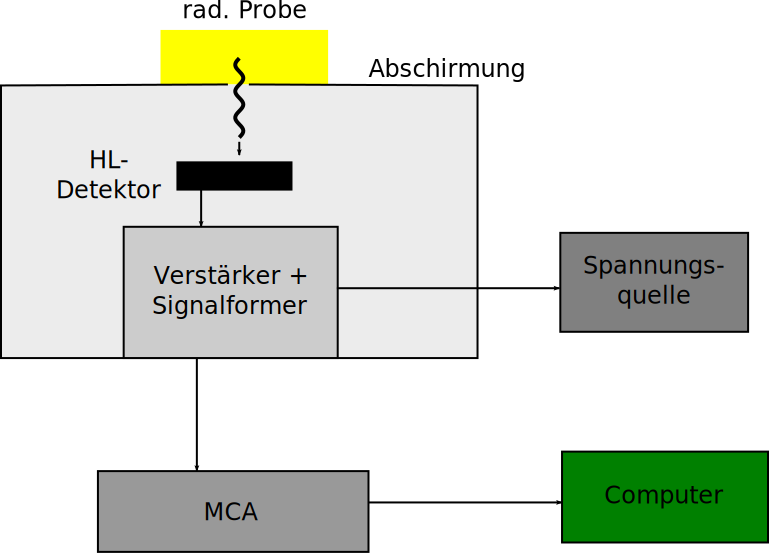
\includegraphics[width=0.7\textwidth]{../img/aufbauHD.pdf}
  \caption{Aufbau zur Messung des Strahlungsspektrums einer radioaktiven Probe mit einem Halbletierdetektor.}
  \label{img:aufbauHD}
\end{center}
\end{figure}
\autoref{img:aufbauHD} zeigt, wie mit einem Halbleiterdetektor Messungen durchgeführt werden.
Er befindet sich zusammen mit Elektronik zur Signalformung in einer abgeschirmten Metallbox.
Die Spannunggsversorgung erfolgt über ein Netzteil.
Auf der Metallbox liegt eine radioaktive Probe, deren Strahlung durch ein Loch in der Box auf den Sensor fällt.
Das Ausgangssignal der Elektronik wird von einem MCA ausgewertet und die Daten an den Computer gesendet.